\documentclass[../main.tex]{subfiles}
\begin{document}
\section{避障规划}

\subsection{避障规划的基本概念}
\begin{enumerate}
    \item \textbf{避障规划}:根据所得到的实时传感器测量信息,规划/调整路径/轨迹,以避免发生碰撞。
    \\{\small\kaishu (也称为反应式避障)}
    \item \textbf{主要方法}:
        \begin{itemize}
            \item \hyperref[bug]{BUG算法}
                \begin{itemize}
                    \item \hyperref[bug1]{BUG1}
                    \item \hyperref[bug2]{BUG2}
                \end{itemize}
            \item \hyperref[shichang]{人工势场法}
            \item \hyperref[xiangliang]{向量势直方图法(VFH)}
            \item \hyperref[dynamicwindow]{动态窗口法(DWA)}
        \end{itemize}
\end{enumerate}

\subsection{避障规划算法}
\begin{enumerate}
    \item \textbf{BUG算法}\label{bug}
        \begin{figure}[H]
            \centering
            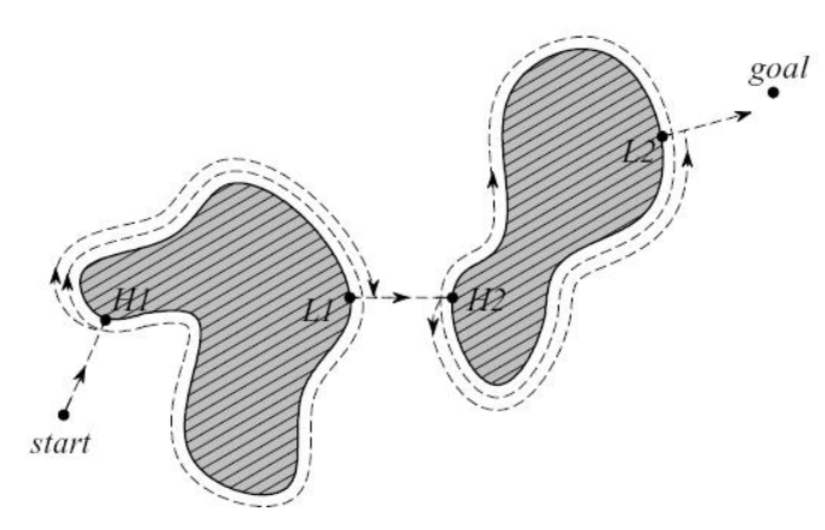
\includegraphics[width=0.4\textwidth]{images/bug.png}
            \caption{BUG算法示意图}
        \end{figure}
        \textbf{基本思想}:让机器人朝着目标前进,当行进路径上出现障碍物时,机器人绕着障碍物的轮廓移动,然后绕离它,继续驶向目标。
        \begin{enumerate}
            \item \textbf{BUG1}\label{bug1}
                    \begin{figure}[H]
                        \centering
                        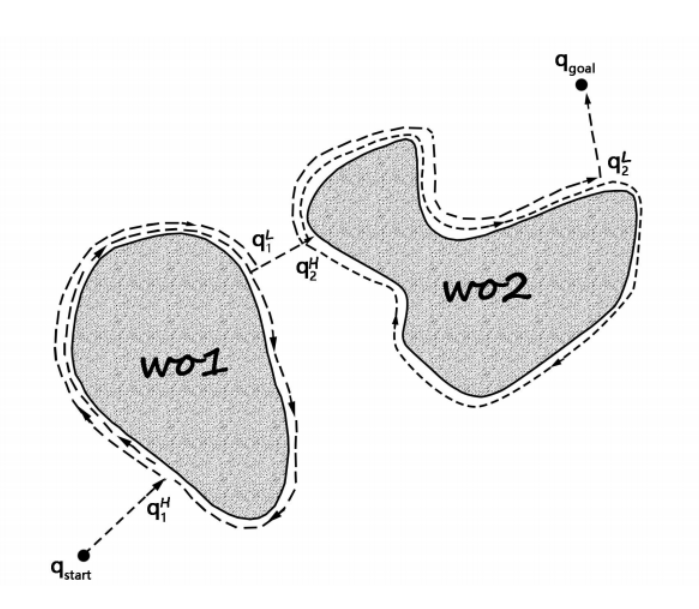
\includegraphics[width=0.4\textwidth]{images/bug1.png}
                        \caption{BUG1算法示意图}
                    \end{figure}
                \begin{itemize}
                    \item \textbf{基本思想}:机器人绕着障碍物轮廓做完整绕行,找出障碍物上最靠近目标点的点,称为离开点(leave point),然后再次绕行到该点,从该点离障碍物,沿直线向目标点移动
                    \item \textbf{绕行距离}:$L \leq d + \dfrac{3}{2} \sum_{i=1}^{N} p_i$
                    \\其中 $d$ 为起始点到目标点的欧氏距离,$p_i$ 为第 $i$ 个障碍物的周长,$N$ 为障碍物个数。
                    \item \textbf{特殊情况}:如果离开点到目标的直线与当前障碍物\textbf{相交},则不存在到达目标的路径。
                        \begin{figure}[H]
                            \centering
                            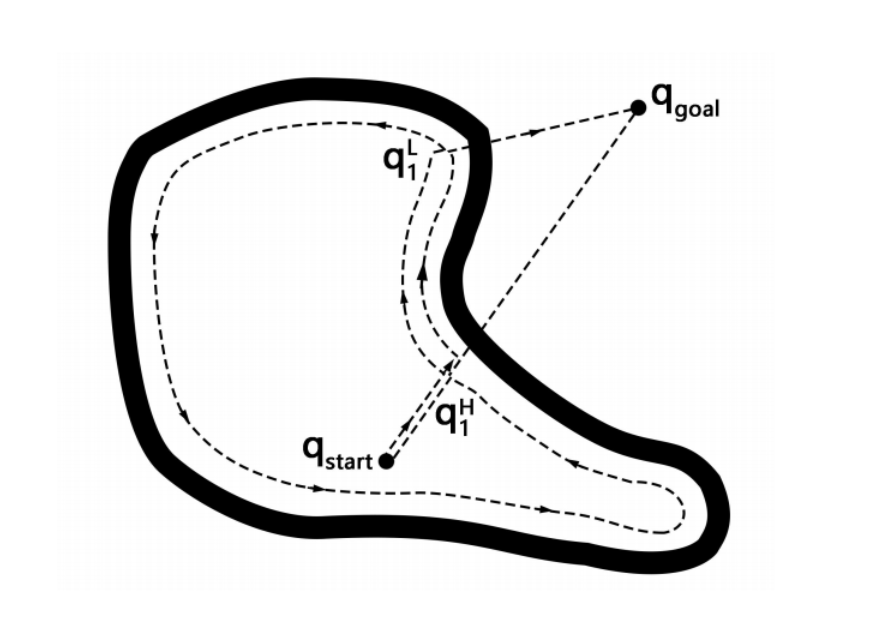
\includegraphics[width=0.4\textwidth]{images/bug1sp.png}
                            \caption{BUG1算法特殊情况}
                        \end{figure}                   
                    \item \textbf{优点}:
                        \begin{itemize}
                            \item 非常简单(可以确保机器人能够到达任何可达目标)
                        \end{itemize}
                    \item \textbf{缺点}:
                        \begin{itemize}
                            \item 效率:为了找到障碍物上最靠近目标的点,需要先绕着障碍物移动一周,效率很低
                        \end{itemize}
                \end{itemize}
            \item \textbf{BUG1}\label{bug2}
                    \begin{figure}[H]
                        \centering
                        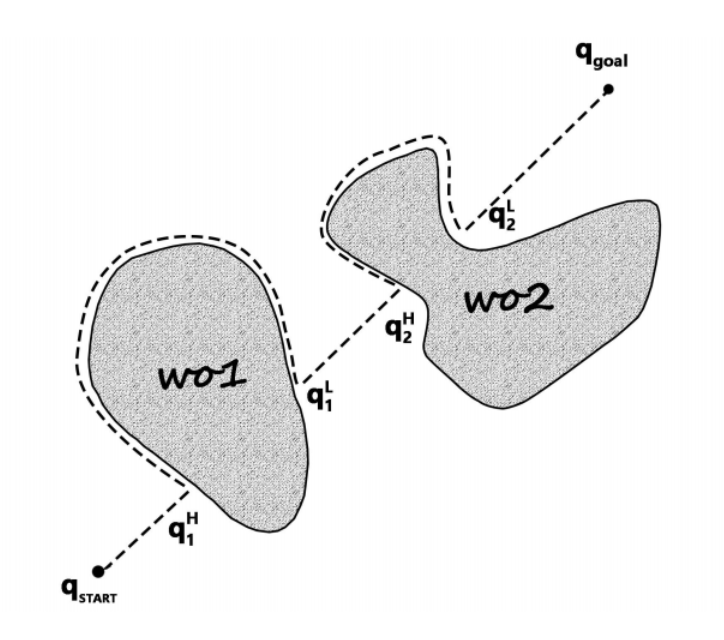
\includegraphics[width=0.4\textwidth]{images/bug2.png}
                        \caption{BUG2算法示意图}
                    \end{figure}
                \begin{itemize}
                    \item \textbf{基本思想}:根据起始点和终止点定义路径L,机器人沿着L行走,当遇到障碍物时,机器人进入障碍物\textbf{轮廓跟踪}模式,\textbf{当到达L上一个接近目标点的位置时,如果该位置比碰到障碍物的位置更接近目标点},则继续沿着L移向目标点,否则继续绕行。
                    \item \textbf{特殊情况}:如果机器人在\textbf{跟踪模式}下再次到达\textbf{进入障碍物轮廓跟踪模式的点},则可以判断不存在到达目标点的路径
                        \begin{figure}[H]
                            \centering
                            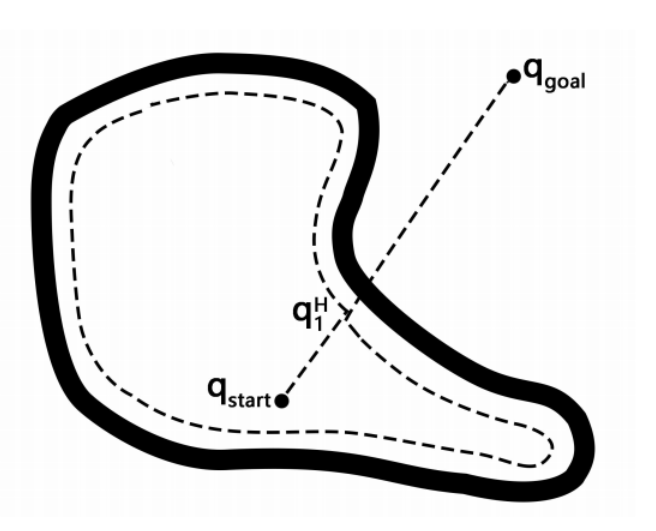
\includegraphics[width=0.4\textwidth]{images/bug2sp.png}
                            \caption{BUG2算法特殊情况}
                        \end{figure}                   
                    \item \textbf{优点}:
                        \begin{itemize}
                            \item 具有较短的移动路径
                        \end{itemize}
                    \item \textbf{缺点}:
                        \begin{itemize}
                            \item 效率:采用贪婪搜索策略,某些情况下移动低效
                        \end{itemize}
                \end{itemize}
                \begin{figure}[htbp]
                    \centering
                    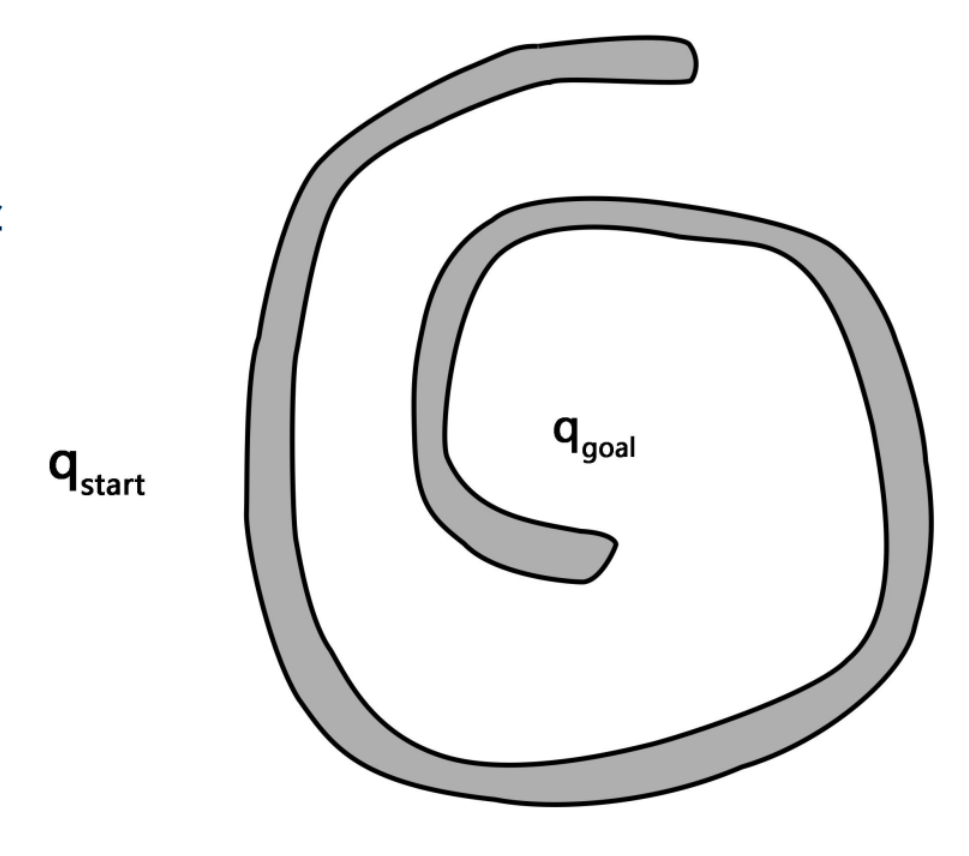
\includegraphics[width=0.35\textwidth]{images/bug2bad.png}
                    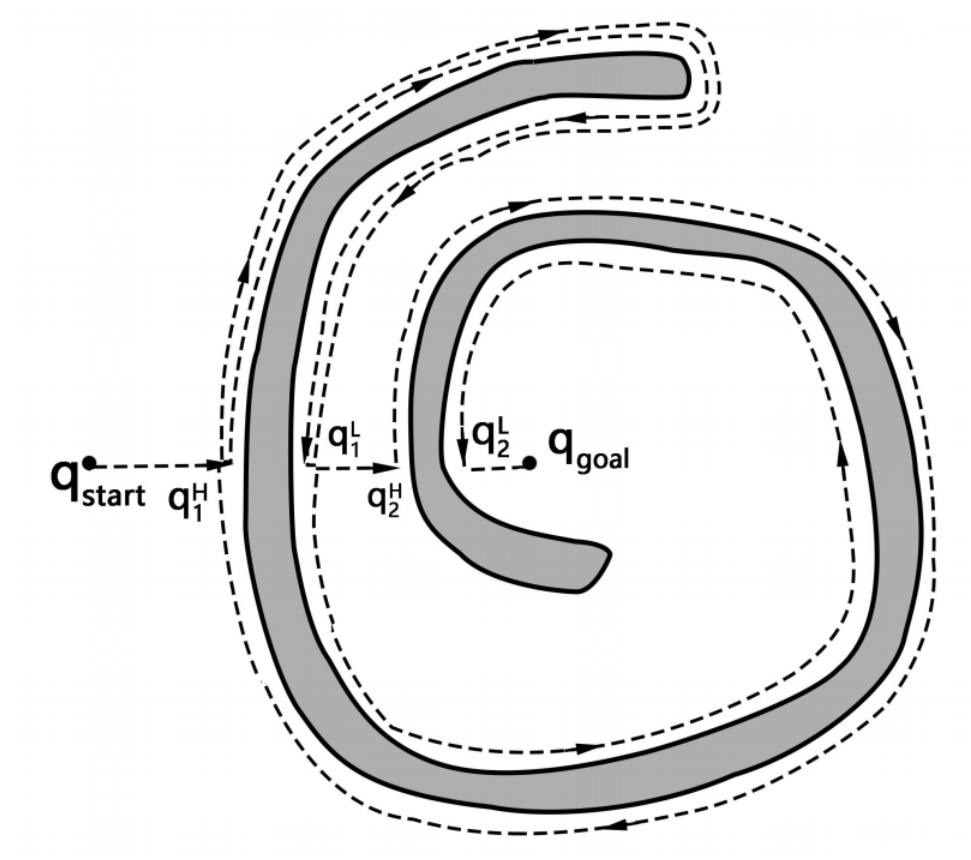
\includegraphics[width=0.35\textwidth]{images/bug2bad2.png}
                    \caption{BUG2算法低效情况示意图}
                    \label{fig:bug2bad}
                \end{figure}
        \end{enumerate}
    \item \textbf{向量势直方图法(VFH)}\label{xiangliang}
        \begin{figure}[H]
            \centering
            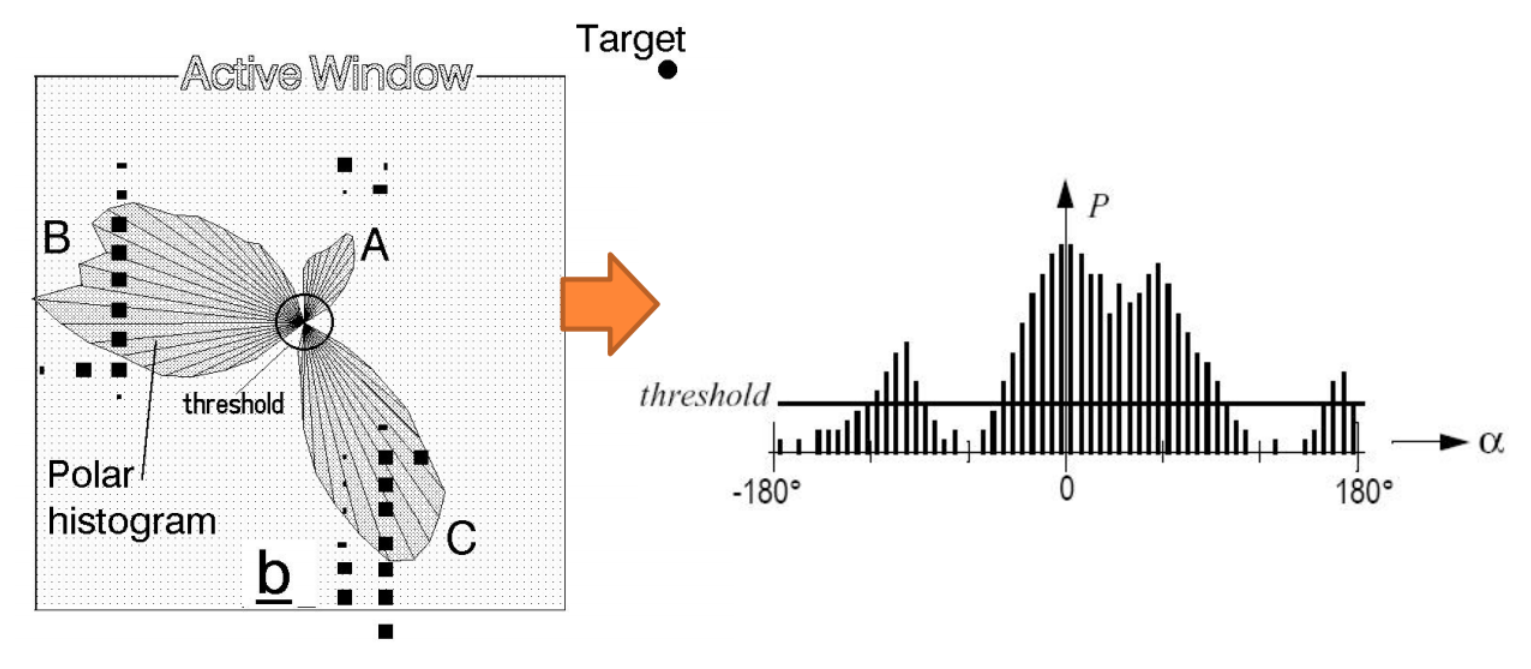
\includegraphics[width=0.3\textwidth]{images/xiangliang.png}
            \caption{VFH算法示意图}
        \end{figure}    
        \begin{itemize}
            \item \textbf{针对问题}:势场法容易陷入局部最优,导致存在振荡、难以通过窄通道,丢失局部障碍物分布详细信息
            \item \textbf{基本思想}:根据环境详细栅格地图构建机器人坐标系下障碍物概率直方图,根据概率直方图评估选择最优运动方向
                \begin{figure}[htbp]
                    \centering
                    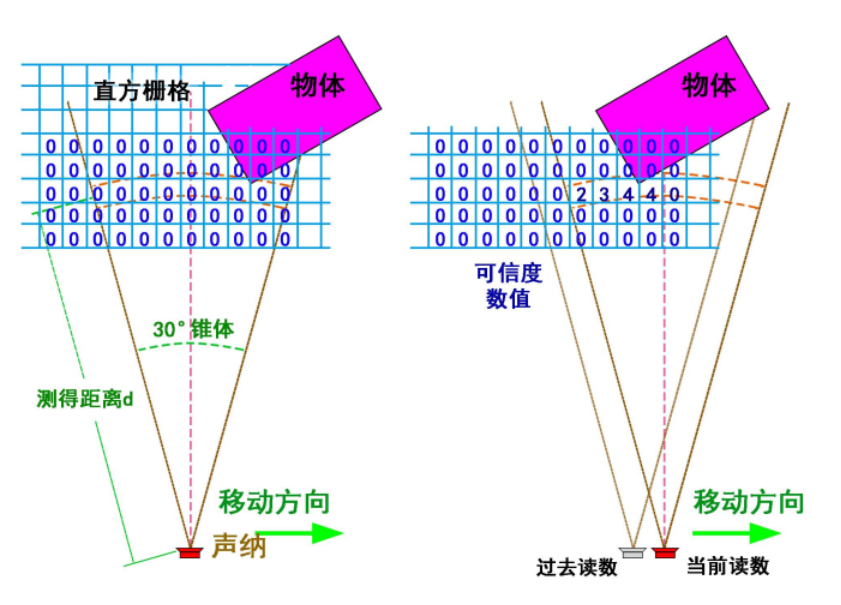
\includegraphics[width=0.35\textwidth]{images/VFM1.png}
                    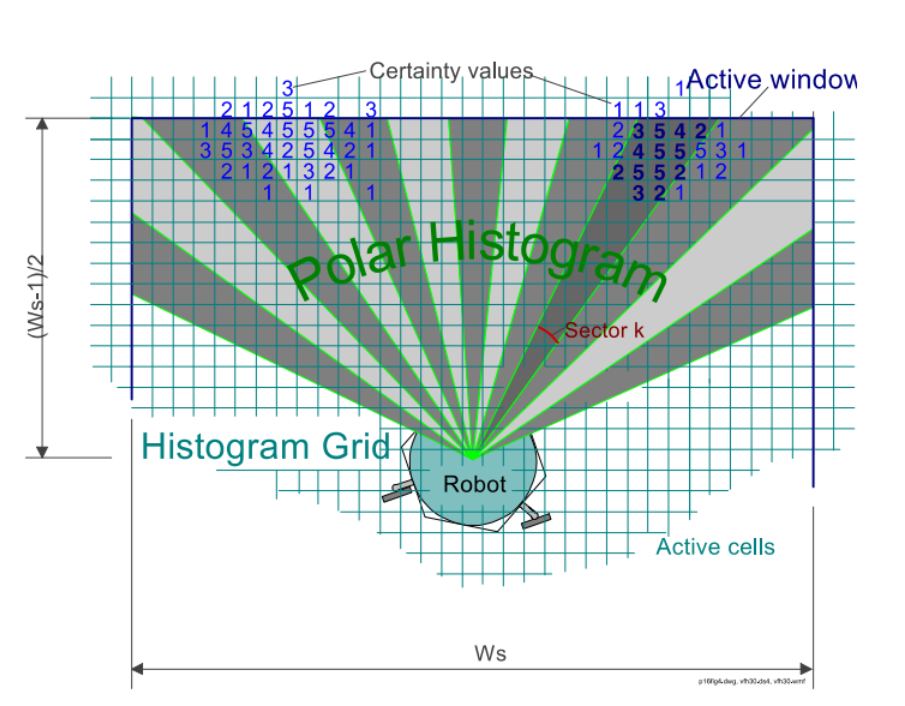
\includegraphics[width=0.35\textwidth]{images/VFM2.png}
                    \caption{VFM构建栅格地图并计算障碍物向量}
                    \label{fig:bug2bad}
                \end{figure}
            \item \textbf{实现步骤}:
                \begin{enumerate}
                    \item \textbf{构建并维护局部栅格地图}
                        \begin{itemize}
                            \item {\small\kaishu 利用距离传感器数据更新机器人周围的栅格地图。}
                            \item {\small\kaishu 根据传感器检测结果,对相应栅格的占用概率进行更新(检测到障碍则栅格值加1)}。
                        \end{itemize}
                    \item \textbf{计算每个栅格的障碍物向量}  
                        \begin{itemize}
                            \item {\small\kaishu 对每个栅格单元计算其与机器人之间的方向与距离:  
                                \[
                                \beta_{i,j} = \tan^{-1}\left(\frac{y_i - y_0}{x_i - x_0}\right)
                                \]
                            \item 向量大小根据栅格可信度和距离确定:  
                                \[
                                m_{i,j} = (c_{i,j}^*)^2 (a - b d_{i,j})
                                \]
                            \item 距离越近、可信度越高的障碍物,其向量值越大。  }
                        \end{itemize}
                    
                    \item \textbf{转换为极坐标下的障碍物概率直方图}  
                        \begin{itemize}
                            \item {\small\kaishu 将0°–360°范围划分为$n$个扇区(分辨率为$\alpha$)。}  
                            \item {\small\kaishu 每个栅格按其方向$\beta_{i,j}$归入对应扇区$k = \text{int}(\beta_{i,j}/\alpha)$。  }
                            \item {\small\kaishu 扇区障碍密度为:}
                                \[
                                h_k = \sum m_{i,j}
                                \]
                            \item {\small\kaishu 对直方图进行平滑处理,减少离散误差。\footnote{由于直方栅格地图的离散特性,为避免一维极坐标系直方图参差不齐影响方向选择,可进行平滑}}  
                        \end{itemize}
                    
                    \item \textbf{根据直方图识别可通行通道并计算导航方向}  
                        \begin{itemize}
                            \item {\small\kaishu 识别所有障碍密度低于阈值的通道。}  
                            \item {\small\kaishu 对每个通道计算综合成本:  }
                                \[
                                G = a \cdot \text{target\_direction} + b \cdot \text{wheel\_orientation} + c \cdot \text{previous\_direction}
                                \]
                            \item {\small\kaishu 其中:}
                                \begin{itemize}
                                {\small\kaishu 
                                    \item \textbf{target\_direction}:路径与目标之间的夹角;
                                    \item \textbf{wheel\_orientation}:新方向与当前机器人朝向的夹角;
                                    \item \textbf{previous\_direction}:上一次选择方向与新方向的夹角。}
                                \end{itemize}
                            \item {\small\kaishu 选择成本最低的通道作为机器人导航方向。  }
                        \end{itemize}
                \end{enumerate}
        \end{itemize}
    \item \textbf{动态窗口法(DWA)}\label{dynamicwindow}
        \begin{figure}[H]
            \centering
            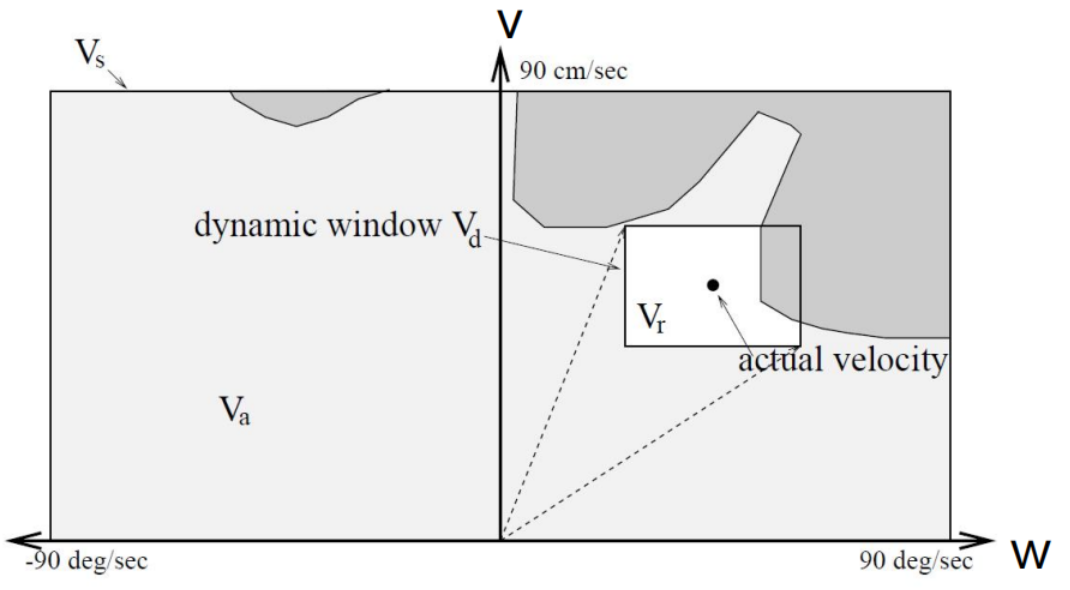
\includegraphics[width=0.4\textwidth]{images/dwa.png}
            \caption{DWA算法示意图}
        \end{figure}
        \begin{itemize}
            \item \textbf{基本思想}:在速度空间中搜索适当的平移速度和旋转速度指令$(v,\omega)$\footnote
            \item \textbf{搜索空间}:速度空间\footnote{之前的方法是几何空间搜索,这里转化为了速度空间搜索}
            \item \textbf{实现步骤}:
                \begin{enumerate}
                    \item 可行空间确定:基于速度控制运动模型\footnote{例如,假如没有噪声,定义控制时间间隔是$\Delta t$,假设$\Delta t$内机器人线速度、角速度保持不变,做一个半径为$r=\frac{v}{\omega}$的圆周运动。},构建\textbf{可行的速度空间}\footnote{不同的速度指令$(v,\omega)$会得到不同运动半径,同样的时间间隔$\Delta t$会到达不同的终止位置,有些是安全的,也就是可行的。}
                        \begin{itemize}
                            \item {\small\kaishu 在速度控制模型下,机器人在$\Delta t$时间间隔内若线速度$v$与角速度$\omega$保持不变,则位置变化为:}
                            \[
                            \begin{cases}
                            x' = x - \frac{v}{\omega}\sin(\theta) + \frac{v}{\omega}\sin(\theta + \omega \Delta t) \\
                            y' = y + \frac{v}{\omega}\cos(\theta) - \frac{v}{\omega}\cos(\theta + \omega \Delta t) \\
                            \theta' = \theta + \omega \Delta t
                            \end{cases}
                            \]
                            \item {\small\kaishu 根据该模型,可定义使机器人不与障碍物相撞的可行速度集合:}
                            \[
                            V_a = \left\{(v,\omega)\, \middle|\, v \le \sqrt{2 \times dist(v,\omega) \times \dot{v}_b}\ \cup\ \omega \le \sqrt{2 \times dist(v,\omega) \times \dot{\omega}_b}\right\}
                            \]
                            \item {\small\kaishu 其中 $dist(v,\omega)$ 表示该速度对应轨迹上距离最近障碍物的距离;$\dot{v}_b$、$\dot{\omega}_b$ 分别为刹车平移与旋转加速度。}
                        \end{itemize}
                
                    \item 窗口空间确定:考虑到机器人在运动过程中\textbf{最大加速度}的约束,在当前速度配置处以\textbf{固定的小时间间隔}开一个速度窗口空间
                        \begin{itemize}
                            \item {\small\kaishu 考虑机器人最大线加速度$a_{v_{\max}}$和最大角加速度$a_{\omega_{\max}}$,其可达速度范围定义为:}
                            \[
                            V_d = \{(v,\omega)\,|\,v \in [v_l,v_h] \wedge \omega \in [\omega_l,\omega_h]\}
                            \]
                            \item {\small\kaishu 其中各边界为:}
                            \[
                            \begin{cases}
                            v_l = v_a - a_{v_{\max}} \times \Delta t, \quad v_h = v_a + a_{v_{\max}} \times \Delta t \\
                            \omega_l = \omega_a - a_{\omega_{\max}} \times \Delta t, \quad \omega_h = \omega_a + a_{\omega_{\max}} \times \Delta t
                            \end{cases}
                            \]
                            \item {\small\kaishu 该集合反映了机器人在$\Delta t$时间内可通过加减速达到的速度范围。}
                        \end{itemize}
                
                    \item 结合机器人速度约束,获得可行速度空间为
                        \begin{itemize}
                            \item {\small\kaishu 结合机器人结构及电机极限,定义最大允许速度范围:}
                            \[
                            V_s = \{(v,\omega)\,|\,v \in [-v_{\max},v_{\max}] \wedge \omega \in [-\omega_{\max},\omega_{\max}]\}
                            \]
                            \item {\small\kaishu 最终可行速度空间为三个集合的交集:}
                            \[
                            V_r = V_a \cap V_d \cap V_s
                            \]
                            \item {\small\kaishu 该空间内的速度对保证了安全性、动态约束及硬件限制同时满足。}
                        \end{itemize}
                
                    \item 在可行速度空间中选择最优的速度控制指令
                        \begin{itemize}
                            \item {\small\kaishu 对每一对候选$(v,\omega)$,定义评价函数:}
                            \[
                            evaluation(v,\omega) = \alpha \cdot heading(v,\omega) + \beta \cdot dist(v,\omega) + \gamma \cdot velocity(v,\omega)
                            \]
                            \item {\small\kaishu 其中 $\alpha + \beta + \gamma = 1, \ \alpha,\beta,\gamma \ge 0$。}
                            \item {\small\kaishu 各项意义如下:}
                                \begin{itemize}
                                    {\small\kaishu 
                                    \item $heading(v,\omega)$:朝向目标点,保证机器人朝目标运动;
                                    \item $dist(v,\omega)$:远离障碍物,保证安全;
                                    \item $velocity(v,\omega)$:速度最大化,保证高效运动。}
                                \end{itemize}
                            \item {\small\kaishu 对三个分量进行\textbf{归一化处理}后,选取评价值最高的$(v,\omega)$作为最优控制指令。}
                        \end{itemize}
                \end{enumerate}

            \item \textbf{缺点}:
                \begin{itemize}
                    \item 运动:据单步信息数据计算期望速度,在评估选择速度时不考虑速度和路径平滑,容易导致机器人运动存在震动和轨迹扭动问题
                    \item 适应性:参数较多,实际实现依赖工程经验,难以适应各种情况
                \end{itemize}
        \end{itemize}


\begin{table}[H]
    \centering
    \small
    \begin{tabular}{
        >{\centering\arraybackslash}m{4cm}
        >{\centering\arraybackslash}m{5.5cm}
        >{\centering\arraybackslash}m{5.5cm}
    }
        \toprule
        \textbf{比较维度} & \textbf{向量势直方图法} & \textbf{动态窗口法} \\
        \midrule
        目标函数构建 & 
        \makecell[{{p{5.5cm}}}]{路径与目标对齐量 \\ 新方向和机器人方向的差异量 \\ 原来选择方向和新方向之间的差异量} &
        \makecell[{{p{5.5cm}}}]{朝向目标点 \\ 远离障碍物 \\ 速度最大化} \\
        \midrule
        是否需要归一化 & 否\footnote{三个量都是角度量,因此不需要做归一化} & 是 \\
        \bottomrule
    \end{tabular}
    \caption{VFH与DWA在目标函数上的对比}
\end{table}


    \end{enumerate}
\end{document}